\documentclass[dvipdfmx]{standalone}
\usepackage{graphicx}
\usepackage{amsmath,amssymb}
\usepackage{tikz}
\usetikzlibrary{calc, arrows.meta}

\begin{document}
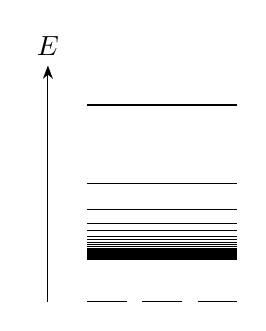
\begin{tikzpicture}
    \draw[->, >=Stealth](0,-.0)--(0,3)node[above]{$E$};
    \draw(.5,0)--(1,0);
    \draw(1.2,0)--(1.7,0);
    \draw(1.9,0)--(2.4,0);
    \foreach\y in{1,2,...,50}{
        \draw(.5,{2/\y+.5})--(2.4,{2/\y+.5});
    }
\end{tikzpicture}
\end{document}